\RequirePackage{luatex85}
\documentclass{standalone}
\usepackage{amssymb,amsmath}
\usepackage{tikz}
\usetikzlibrary{automata,positioning}
\begin{document}
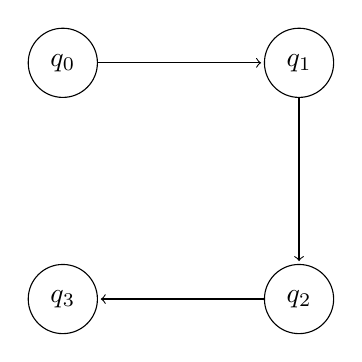
\begin{tikzpicture}[shorten >=1pt,node distance=3cm,on grid,auto] 
 \node[state] (q_0) {$q_0$};
 \node[state] (q_1)[right=of q_0] {$q_1$};
 \node[state] (q_2)[below=of q_1] {$q_2$};
 \node[state] (q_3)[below=of q_0] {$q_3$};
 \path[->]
 (q_0) edge (q_1)
 (q_1) edge (q_2)
 (q_2) edge (q_3);
\end{tikzpicture} 
 \end{document}